\documentclass{article}

\usepackage[utf8]{inputenc}

\usepackage{amsmath}
\usepackage{graphicx}
\usepackage{amssymb}
\usepackage{float}
\usepackage{caption}
\usepackage{subcaption}

\setlength{\parskip}{\baselineskip}%
\setlength{\parindent}{0pt}%

\begin{document}

\title{Boundary Layers}
\author{lwp26 }
\date{October 2022}
\maketitle

\section{Abstract}

\section{Introduction}

% Aims, Objectives and context
\subsection{Importance of packaging materials}

\subsection{Aims}

\begin{itemize}
\item To develop a method for selecting packing foam materials for given applications
\item 
\end{itemize}

\section{Methodology}

We compressed various foams to determine their elastic moduli


\section{Results}


\subsection{Foam properties}

\begin{figure}[H]
\centering
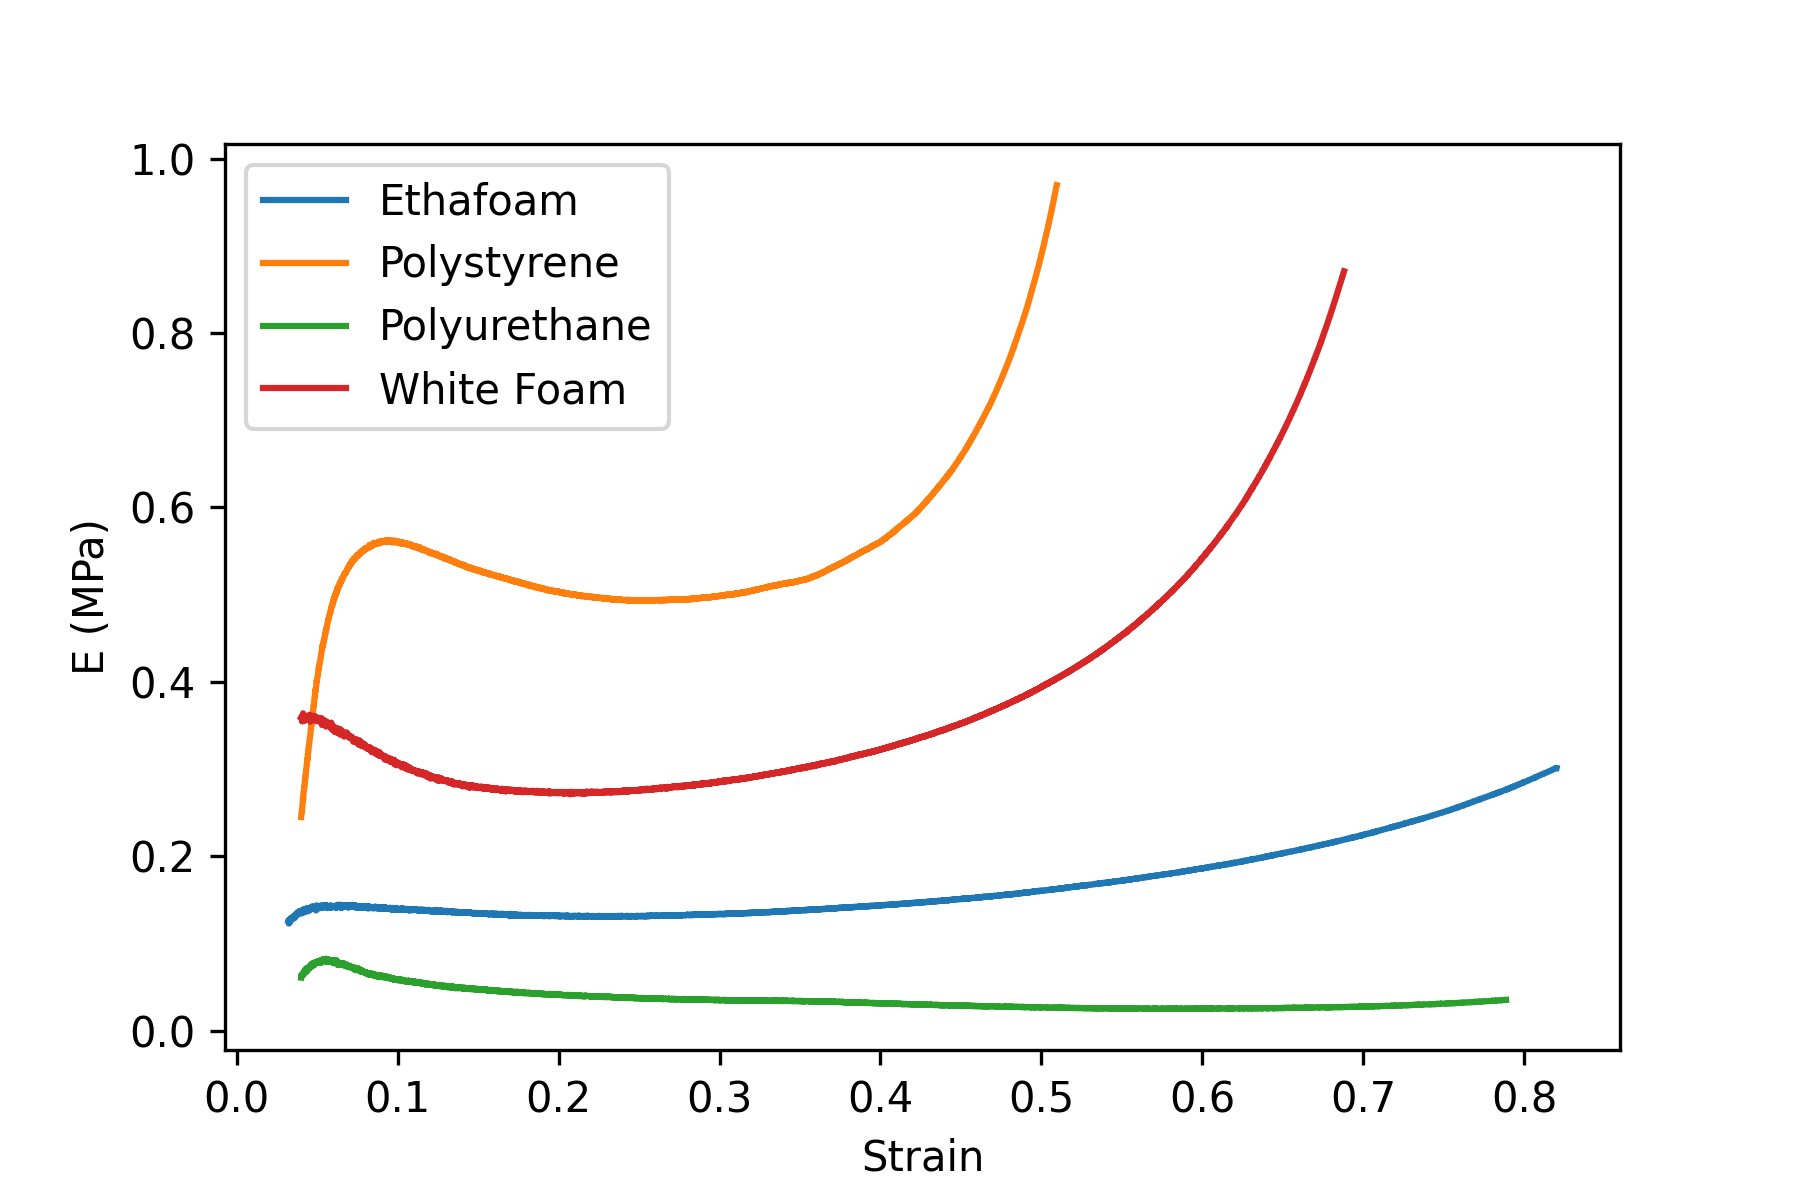
\includegraphics[width=1\textwidth]{E_vs_strain.png}
\caption{\label{fig:E_strain} Graph of the laminar and turbulant flow profiles}
\end{figure}


\subsection{Foam images}

\begin{figure}[H]
\centering
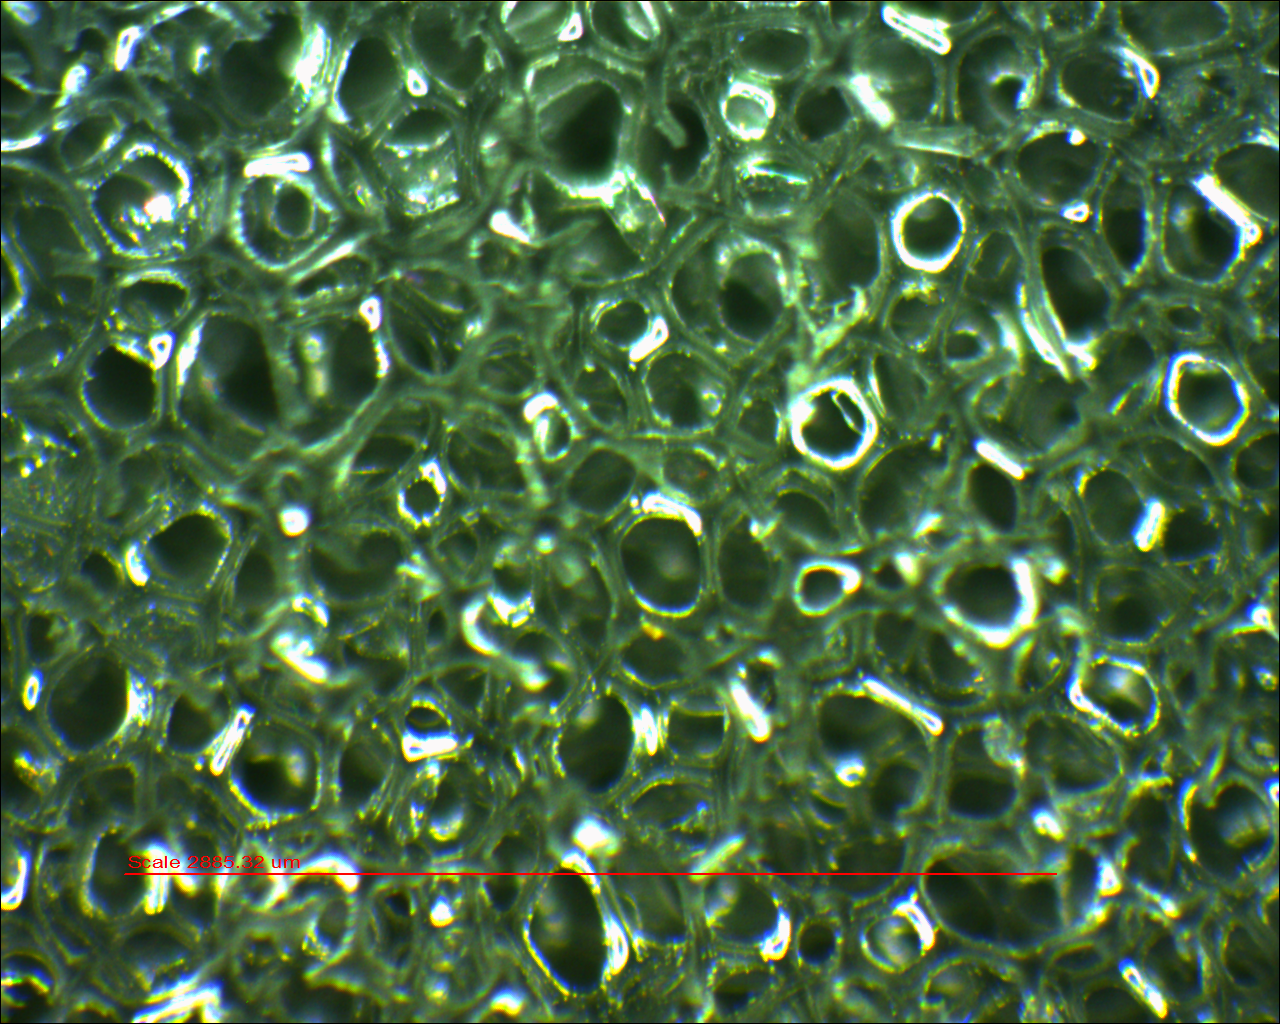
\includegraphics[width=0.8\textwidth]{17_polyurethane.png}
\caption{\label{fig:polyurethane} Polyurethane foam}
\end{figure}

\begin{figure}[H]
\centering
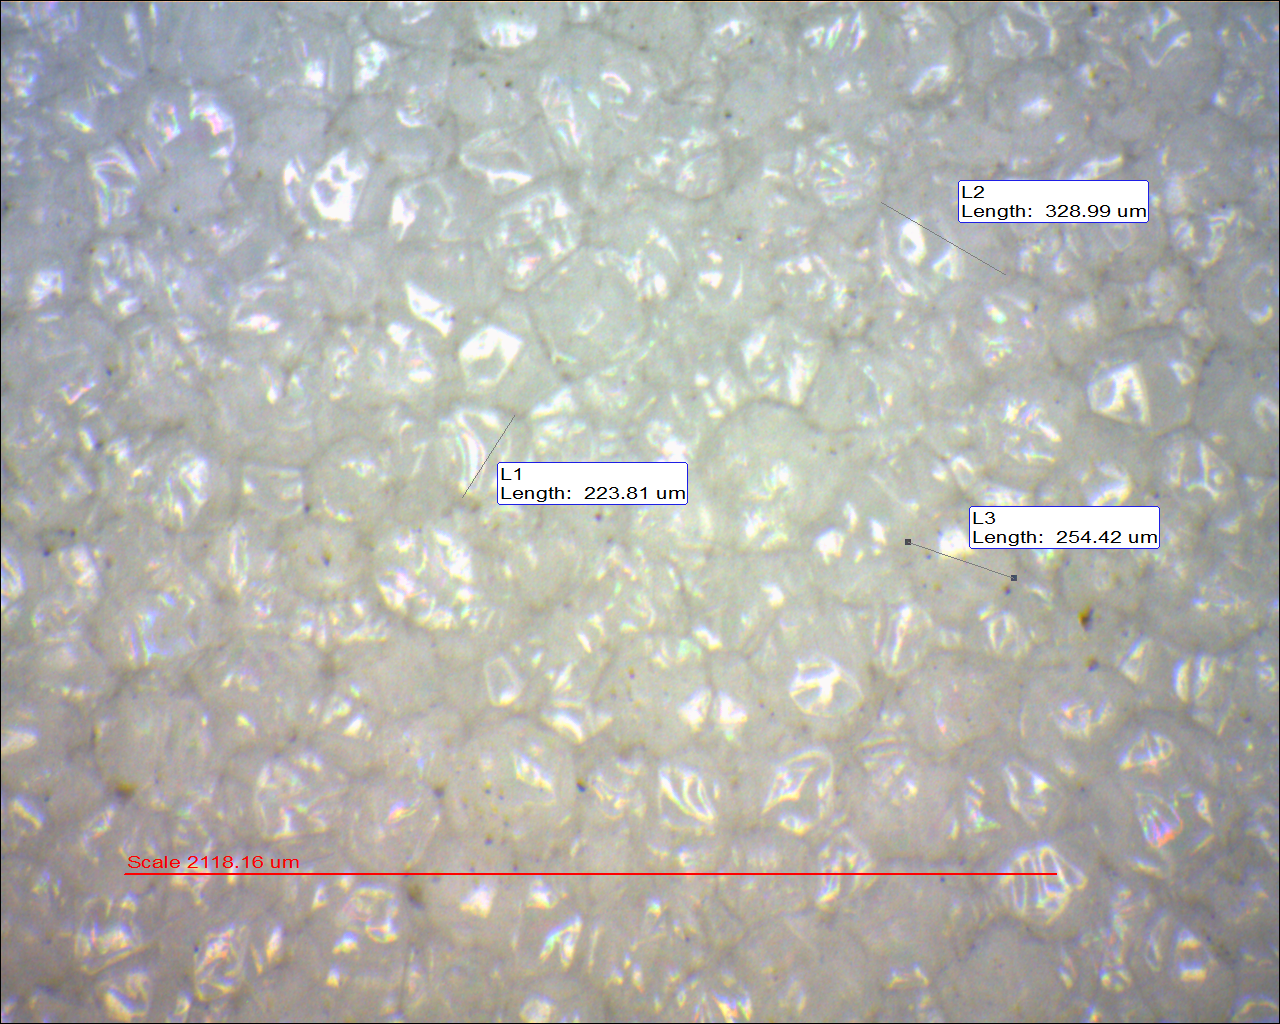
\includegraphics[width=0.8\textwidth]{17_white_foam.png}
\caption{\label{fig:white_foam} Dense white foam}
\end{figure}

\begin{figure}[H]
\centering
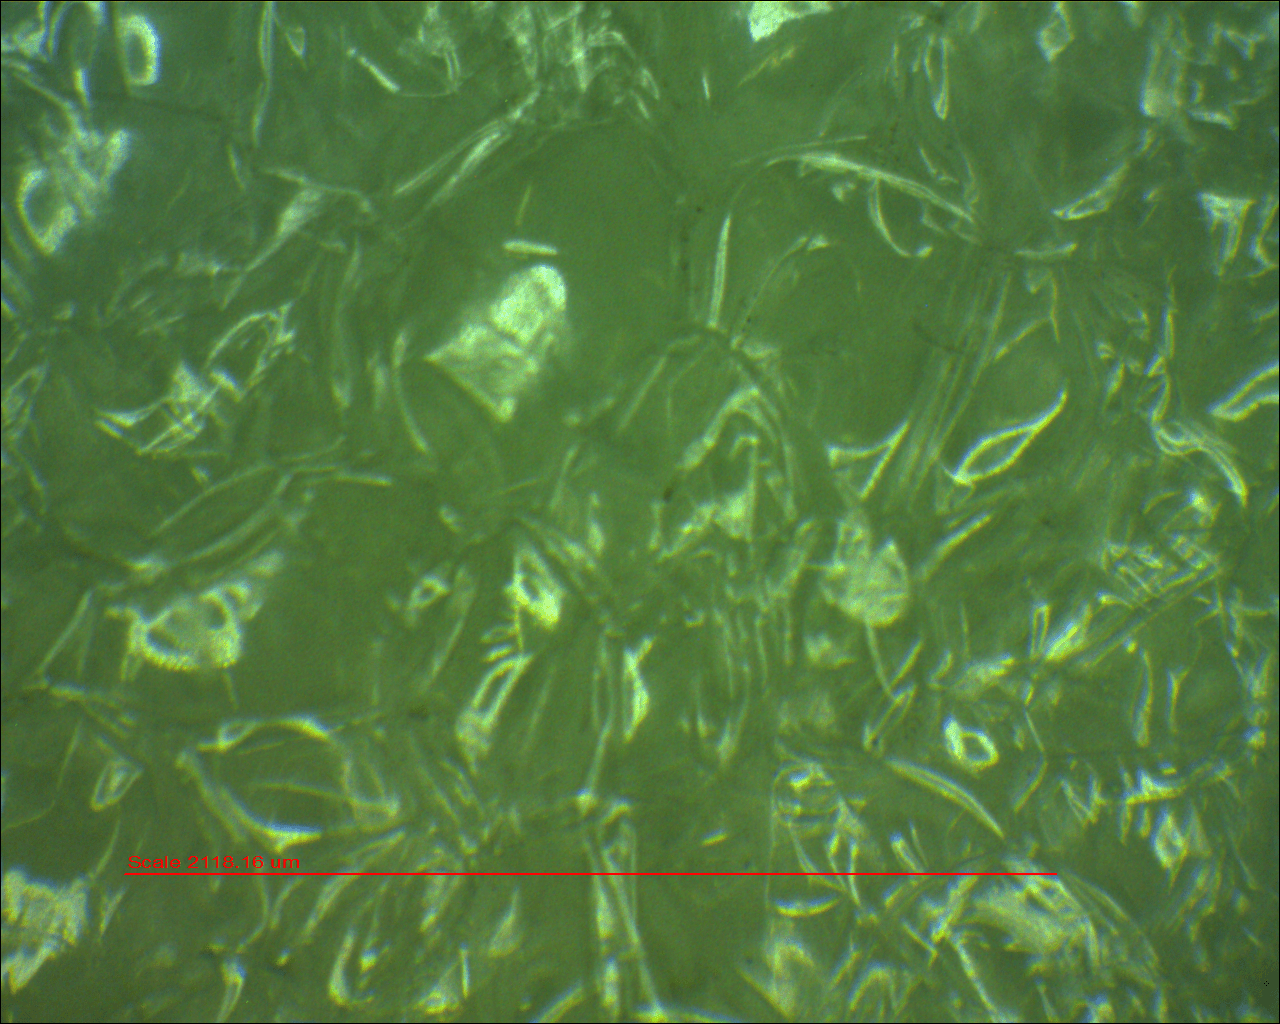
\includegraphics[width=0.8\textwidth]{17_ethafoam.png}
\caption{\label{fig:ethafoam} Ethafoam}
\end{figure}

\begin{figure}[H]
\centering
\subfloat[\centering compressed]{{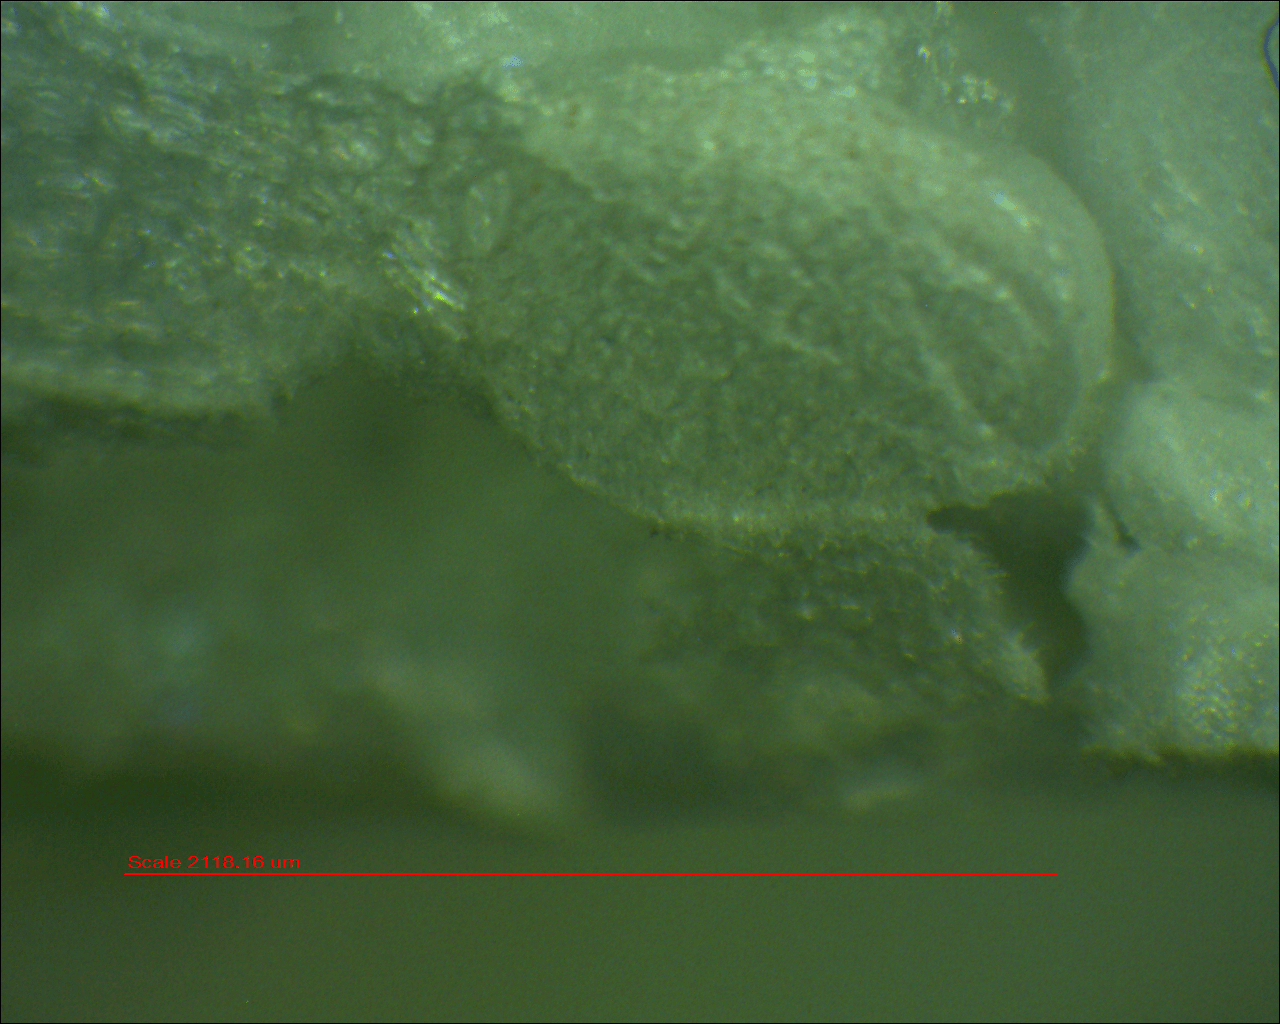
\includegraphics[width=5cm]{17_polystyrene_compressed.png} }}%
\qquad
\subfloat[\centering uncompressed]{{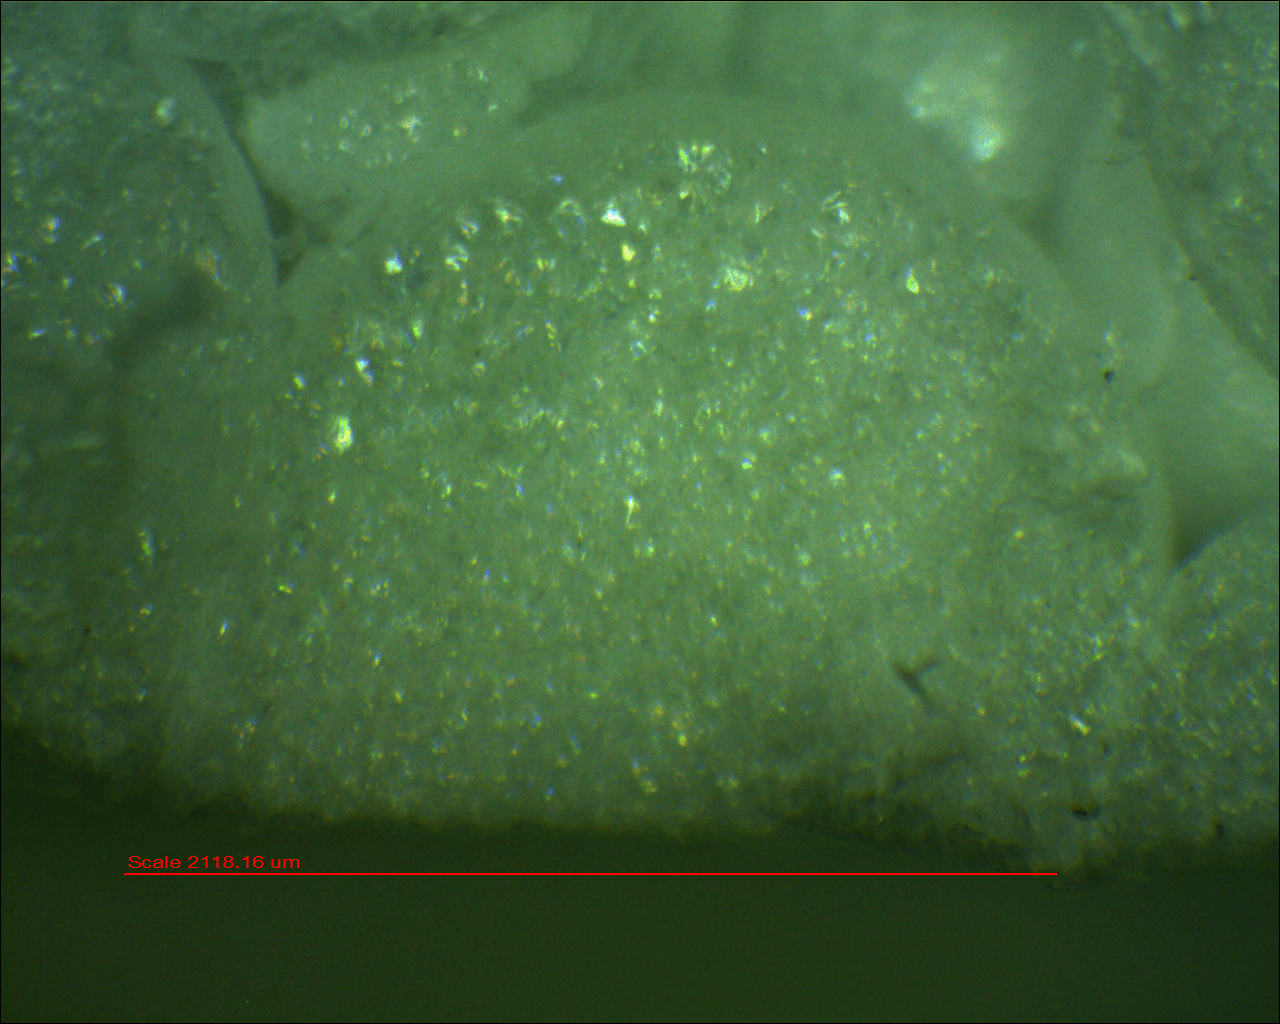
\includegraphics[width=5cm]{17_polystyrene_uncompressed.png} }}%
\caption{\label{fig:polystyrene} Blown polystyrene before and after compression}
\end{figure}

\section{Discussion}

The sudden drop in drag coefficient is due to the boundary layer in front of the sphere becomming thinner and the flow transitions into turbulant 

%interpret results and comment on anomalies

\section{Conclusion}

In conclusion

\end{document}